\documentclass[12pt]{article}
%\usepackage{epsf,epic,eepic,eepicemu}
%\documentstyle[epsf,epic,eepic,eepicemu]{article}
%\usepackage[cp1250]{inputenc}
\usepackage[utf8]{inputenc}
\usepackage[czech, english]{babel}
\usepackage{czech}
\usepackage[T1]{fontenc} 
\usepackage{verbatim}
\usepackage{graphicx}
\usepackage{hyperref}
\usepackage{lmodern}
\usepackage{float}

\makeindex

\begin{document}
%\oddsidemargin=-5mm \evensidemargin=-5mm \marginparwidth=.08in
%\marginparsep=.01in \marginparpush=5pt \topmargin=-15mm
%\headheight=12pt \headsep=25pt \footheight=12pt \footskip=30pt
%\textheight=25cm \textwidth=17cm \columnsep=2mm \columnseprule=1pt
%\parindent=15pt\parskip=2pt

\begin{center}
\bf Semestrální projekt MI-PAP 2010/2011:\\[5mm]
    Paralelní řadící algoritmy\\[5mm]
    Pavel Benáček\\   
    Tomáš Čejka\\[2mm]
magisterské studijum, FIT ČVUT, Kolejní 550/2, 160 00 Praha 6\\[2mm]
\today
\end{center}
\newpage

\tableofcontents
\listoftables
\newpage
\section{Definice problému a popis sekvenčního algoritmu}
\subsection{Zadání}
Podle zadání semestrální práce je úkolem implementace aspoň tří z následujících
řadících algoritmů: Shearsort, 3D sort, Sudo-lichý Mergesort a Bitonic sort.

Pro řešení jsme si vybrali algoritmy Shearsort, Sudo-lichý Mergesort a Bitonic sort.

Pro účely měření času běhu výsledných programů a porovnání paralelních algoritmů se sekvenčním
řazením jsme si implementovali sekvenční algoritmus Mergesort a ten vzali jako referenční sekvenční
řešení.

Semestrální práce spočívala v implementaci vybraných řadících algoritmů jako sekvenční řešení, paralelní
řešení na počítači se sdílenou pamětí s použítím knihovny OpenMP a následně s využitím technologie CUDA
společnosti NVIDIA\textsuperscript{\tiny{\textregistered}}.

\label{sec:reseni}
\subsection{Řešení}
Algoritmy byly ve své podstatě navrženy tak, aby co nejlépe seděli možnostem a architektuře CUDA. Bylo dbáno na několik základních vlastností. A to:
\begin{itemize}
	\item co největší počet vláken v bloku
	\item co nejvíce nezávislých bloků
	\item minimalizace komunikace do globální paměti
\end{itemize}

Tyto části jsou společné pro všechny algoritmy pro CUDA. Zaručují jistou rychlost a škálovatelnost problému.

\section{Popis paralelního algoritmu a jeho implementace v CUDA}
\subsection{Shearsort}
Vzhledem k možnosti HW v grafickém akcelerátoru jsme zvolili implementaci pomoci even odd transpozition sortu. Toto využívání je možné zejména díky schopnosti vytvořit velký počet vláken v zařízení (a to,že každý prvek v poli má své vlastní vlákno). Při samotné implementaci bylo dbáno na několik základních pravidel. A to pravidla v úvodní části \ref{sec:reseni}.

Po nastartování kernelu se provede nakopírování dat do sdílené paměti. Samotné řazení probíhá ve sdílené paměti a mimo bloková komunikace (výměna) probíhá přez globální paměť (kde komunikaci provádí POUZE prvky na přechodu mezi bloky). 

Samotný shearsort byl implementován jako kernel, tak veškerá část algoritmu běží na GPU. Pro tuto příležitost byl implementován algoritmus synchronizace mezi bloky, který byl popsán v \ref{cud:synblocks}. Tento algoritmus nám umožnil synchronizaci mezi bloky a tak se nemuselo z kernelu vystupovat a provádět synchronizaci bloků v rámci programu hosta.

Program si sám spočítá rozložení matice tak, aby se do globální paměti vlezl celý sloupec 2D matice.

\subsection{Sudo-lichý mergesort, Bitonic sort}
Řešení algoritmů sudo-lichý mergesort a bitonic sort jsme nalezli v ukázkových příkladech, dodávaných společně s SDK, stažitelných
ze stránek společnosti
NVIDIA. Jedná se o příklad pojmenovaný \textbf{sortingNetworks}. Spustitelný program, který se v příkladu generoval, prováděl
řazení pouze algoritmem Bitonic sort. Zdrojový kód v \textbf{main.cpp} jsme proto upravili tak, aby se dal spustit i sudo-lichý mergesort.
Program nyní očekává při spuštění jeden parametr a to buď \emph{bitonic} nebo \emph{eom} a podle toho se použije řadící algoritmus.
SortingNetworks jsme přesunuli z adresářové struktury příkladů tak, aby se dal zkompilovat samostatně a nezávisle na příkladech
a k tomu jsme upravili soubor Makefile.

\section{Naměřené výsledky}
\subsection{Způsob měření}
Měření bylo prováděno nad daty, které se generovalo pro každý každý problém znova a které samozřejmě do doby běhu algoritmu nebylo započítáno. Měření času bylo prováděno prostředky z CUDA SDK. Pro vyhodnocení jsme zvolili konstatní počet vláken na blok.

\subsection{Naměřené časy}
\subsubsection{Shearsort}
\begin{table}[H]
\begin{center}
\begin{tabular}{|r|r|r|}
\hline Množství dat (2\textsuperscript{n}) & Čas \\ \hline
\begin{comment}
4   0.000200800
5   0.000282080
6   0.000556640
7   0.001100000
8   0.002022474
9   0.007240000
10  0.014284000
11  0.016643200
12  0.019943290
13  0.027145500
14  0.043032042
15  0.093929000
16  0.215102000
17  0.702910000
18  2.339670000
19  8.812000000
20  35.23100000
21  166.1040000
22  652.323000 
\end{comment}
4       &  0.000200800 \\ \hline
5       &  0.000282080 \\ \hline
6       &  0.000556640 \\ \hline
7       &  0.001100000 \\ \hline
8       &  0.002022474 \\ \hline
9       &  0.007240000\\ \hline
10      &  0.014284000 \\ \hline
11      &  0.016643200 \\ \hline
12      &  0.019943290 \\ \hline
13      &  0.027145500 \\ \hline
14      &  0.043032042 \\ \hline
15      &  0.093929000 \\ \hline
16      &  0.215102000 \\ \hline
17      &  0.702910000 \\ \hline
18      &  2.339670000 \\ \hline
19      &  8.812000000 \\ \hline
20      &  35.23100000 \\ \hline
21      &  166.1040000 \\ \hline
22	&  652.323000  \\ \hline

\end{tabular} 
\end{center}
\caption{Shearsort}
\end{table} 

\subsubsection{Even-Odd Mergesort}
\begin{table}[H]
\begin{center}
\begin{tabular}{|r|r|r|}
\hline Množství dat (2\textsuperscript{n}) & Čas \\ \hline
\begin{comment}
6  0,000026000
7  0,000006000
8  0,000005000
9  0,000005000
10 0,000004000
11 0,000011000
12 0,000021000
13 0,000033000
14 0,000050000
15 0,000068000
16 0,000091000
17 0,000116000
18 0,000145000
19 0,000176000
20 0,000212000
21 0,000250000
22 0,000291000
24 0,000334000
25 0,000383000
26 0,000433000
27 0,000487000
28 0,000543000
\end{comment}
6  &   0.000026000 \\ \hline
7  &   0.000006000 \\ \hline
8  &   0.000005000 \\ \hline
9  &   0.000005000 \\ \hline
10 &   0.000004000 \\ \hline
11 &   0.000011000 \\ \hline
12 &   0.000021000 \\ \hline
13 &   0.000033000 \\ \hline
14 &   0.000050000 \\ \hline
15 &   0.000068000 \\ \hline
16 &   0.000091000 \\ \hline
17 &   0.000116000 \\ \hline
18 &   0.000145000 \\ \hline
19 &   0.000176000 \\ \hline
20 &   0.000212000 \\ \hline
21 &   0.000250000 \\ \hline
22 &   0.000291000 \\ \hline
24 &   0.000334000 \\ \hline
25 &   0.000383000 \\ \hline
26 &   0.000433000 \\ \hline
27 &   0.000487000 \\ \hline
28 &   0.000543000 \\ \hline
\end{tabular} 
\end{center}
\caption{Even-odd mergesort}
\end{table} 

\subsubsection{Bitonic sort}
\begin{table}[H]
\begin{center}
\begin{tabular}{|r|r|r|}
\hline Množství dat (2\textsuperscript{n}) & Čas \\ \hline
\begin{comment}
6    0,000027000
7    0,000006000
8    0,000005000
9    0,000005000
10   0,000005000
11   0,000040000
12   0,000080000
13   0,000122000
14   0,000167000
15   0,000231000
16   0,000281000
17   0,000323000
18   0,000381000
19   0,000442000
20   0,000510000
21   0,000578000
22   0,000648000
24   0,000721000
25   0,000801000
26   0,000905000
27   0,001000000
28   0,001057000
\end{comment}
6  &   0.000027000  \\ \hline
7  &   0.000006000  \\ \hline
8  &   0.000005000  \\ \hline
9  &   0.000005000  \\ \hline
10 &   0.000005000  \\ \hline
11 &   0.000040000  \\ \hline
12 &   0.000080000  \\ \hline
13 &   0.000122000  \\ \hline
14 &   0.000167000  \\ \hline
15 &   0.000231000  \\ \hline
16 &   0.000281000  \\ \hline
17 &   0.000323000  \\ \hline
18 &   0.000381000  \\ \hline
19 &   0.000442000  \\ \hline
20 &   0.000510000  \\ \hline
21 &   0.000578000  \\ \hline
22 &   0.000648000  \\ \hline
24 &   0.000721000  \\ \hline
25 &   0.000801000  \\ \hline
26 &   0.000905000  \\ \hline
27 &   0.001000000  \\ \hline
28 &   0.001057000  \\ \hline
\end{tabular} 
\end{center}
\caption{Bitonic sort}
\end{table} 


\section{Závěr}
Po seznámení se se základním principem práce s technologií CUDA jsme začali pracovat na paralelizaci řadících algoritmů touto druhou variantou. Oproti použití technologie OpenMP vyžadovala implementace mnohem větší úsilí, takže jsme stihli realizaci algoritmu shearsort. Naštěstí jsme zbylé dva algoritmy našli v příkladech od společnosti NVIDIA, takže pro měření jsme použili mírně modifikované (co do spouštění) tyto implementace.

Technologie CUDA respektive použitá grafická karta nám umožnila využít mnohem více spuštěných vláken oproti např. OpenMP bez nezanedbatelného zvýšení režie, která s použitím vláken v OS souvisí. 
\section{Literatura}
\begin{enumerate}
\item \href{https://edux.fit.cvut.cz/courses/MI-PAP}{Stránky předmětu MI-PAP}
\item \href{http://aggregate.org/MAGIC/#GPU SyncBlocks}{\label{cud:synblocks}GPU synblocks}
\item \href{http://www.root.cz/serialy/uvod-do-technologie-cuda/}{Seriál o technologii CUDA na serveru Root.cz}
\end{enumerate}

\appendix
\section{Grafy závislosti času na velikosti dat}

\subsection{Měření na posloupnosti čísel o velikosti 2\textsuperscript{26}}
\subsubsection{EOMergesort, Bitonic sort}
\begin{figure}[H]
\begin{center}
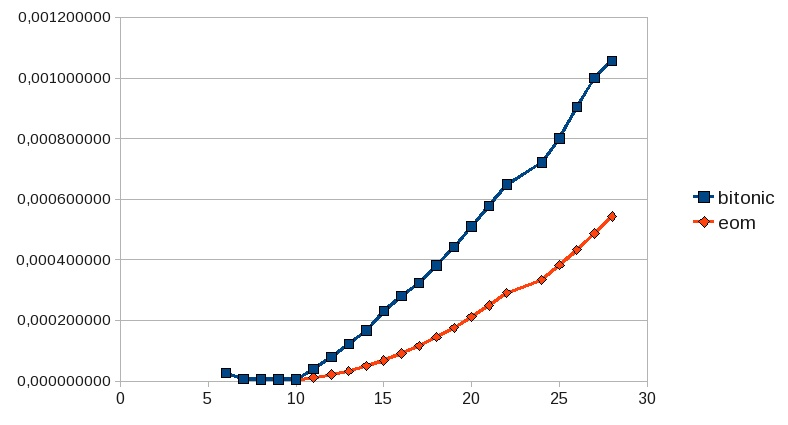
\includegraphics[width=14cm]{cuda-eom-bit.jpg}
\caption{Graf závislosti času na velikosti dat EOMergesort, Bitonic sort}
\label{fig:cuda-eom-bit}
\end{center}
\end{figure}

\subsubsection{Shearsort}
\begin{figure}[H]
\begin{center}
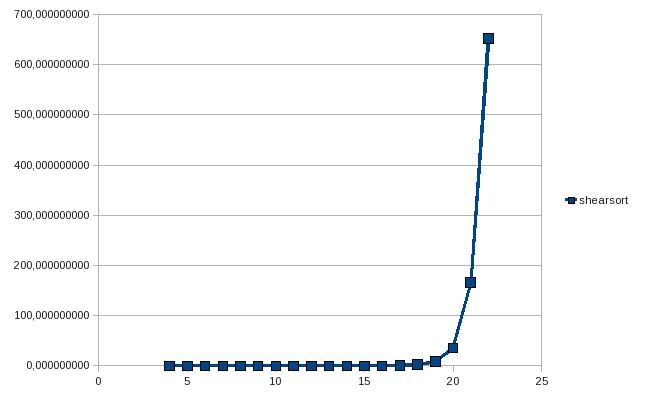
\includegraphics[width=14cm]{cuda-shearsort.jpg}
\caption{Graf závislosti času na velikosti dat Shearsort}
\label{fig:cuda-shearsort}
\end{center}
\end{figure}

\section{Porovnání CUDA a OpenMP}
\subsection{Even-Odd Mergesort}
\begin{figure}[H]
\begin{center}
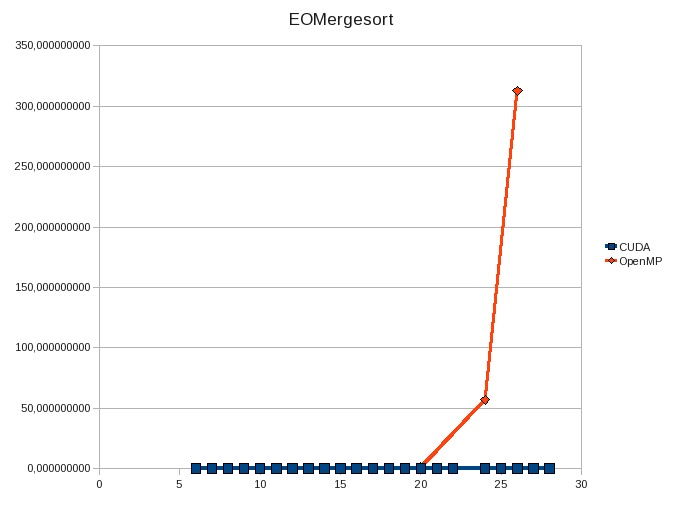
\includegraphics[width=14cm]{eom-cudavsomp.jpg}
\caption{EOMergesort - CUDA vs. OpenMP}
\label{fig:eom-cuda-vs-omp}
\end{center}
\end{figure}

\subsection{Bitonic sort}
\begin{figure}[H]
\begin{center}
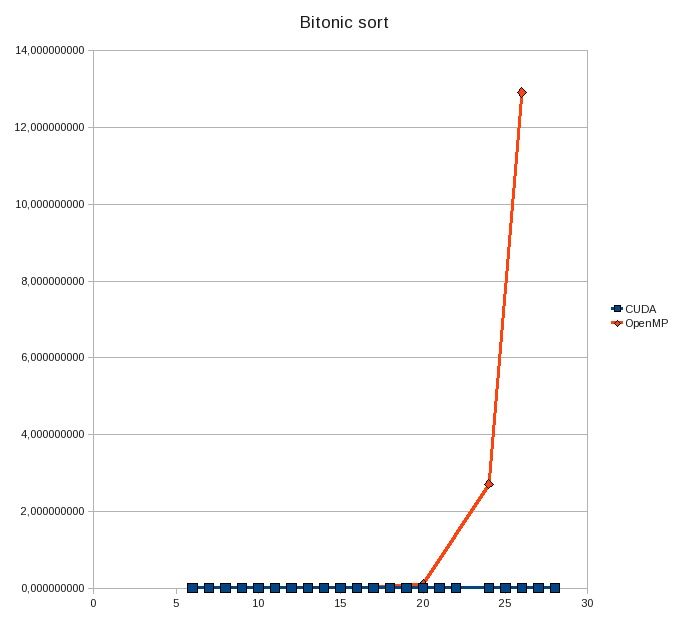
\includegraphics[width=14cm]{bit-cudavsomp.jpg}
\caption{Bitonic sort - CUDA vs. OpenMP}
\label{fig:bit-cuda-vs-omp}
\end{center}
\end{figure}

\subsection{Shearsort}
\begin{figure}[H]
\begin{center}
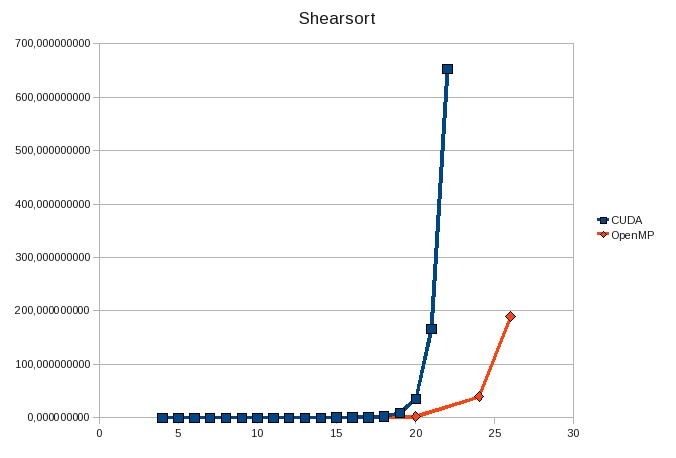
\includegraphics[width=14cm]{shear-cudavsomp.jpg}
\caption{Shearsort - CUDA vs. OpenMP}
\label{fig:shear-cuda-vs-omp}
\end{center}
\end{figure}

\end{document}
